\section{Evaluation}\label{sec:evaluation}
%We describe the design and implementation of HyperPS. 
%In this section, we evaluate the protection effectiveness and performance of HyperPS by exploiting vulnerabilities and comparing it with traditional KVM through a set of benchmarks.
In this section, we first analyze the security guarantees provided by HyperPS. Then, we evaluate the performance overhead by running a set of benchmarks on both standard KVM and HyperPS.



\subsection{Security Analysis}
 
%In section \ref{sec:design}, we discuss in detail how HyperPS achieves memory isolation, and secure interactions between VM and the hypervisor. Just as the threat model described in the section \ref{threat}, an attacker could subvert the upper VMs by conducting attacks such as cross-domain attack with a malicious virtual machine.
In this section, we elaborate the security evaluation on how HyperPS achieves memory isolation among VMs through the monitoring interaction data. 
In addition, we analyze the security of HyperPS itself. Table \ref{tab3} shows the real attack instances in line with the above attack model. 

%However, these two attack vectors, regardless of their attack path, both focus on critical interaction data and data on memory, afterwards, modifying more detailed data, such as the VMCS data structure, EPT and EPT Pointer. Thus, we will elaborate on how HyperPS fends of these attack, and Table \ref{tab3} shows the two real attack instances in line with the above attack model. 
% the attack instances listed in Table \ref{tab3} perfectly match the description of attacker, so we will use these two instances to specifically analyze security performance. 


\textbf{Modifying Interaction-Data Attack}
We clarify interaction data including VMCS in Section \ref{interaction}.
 To prevent interaction-data leakage, we protect VMCS from the attacker. Firstly, VMCS is hidden in HyperPS Space and can not be accessed by hypervisor. Secondly, functions that can access VMCS are hooked into HyperPS Space, therefore, no functions outside HyperPS Space can access VMCS. The attacker can not get location of VMCS and access it. This prevents attackers from tampering interaction data attacks. We examine protection for VMCS by conducting several attack cases which are widely adopted in real world. Table \ref{tab3} lists all attack cases we used. The attack, named Interaction-data attack, tries to tamper the Guest\_CR3 field in VMCS. This attack fails because it can not access VMCS. 
% The experimental results show that the access failed, malicious interaction-data accessing is prevented successfully.
  According to the above analysis, the attacker can not access VMCS, and can not conduct further attacks. Therefore, the VM interaction data can be protected by HyperPS.
  %cannot be modified. 


%CVE-2009-2287 allows attacker to provide invalid value of CR3, which is an important data value in VMCS data structure. Because HyperPS would check the value of CR3 before VM entry instruction is conducted, an attacker has no chance to load the value to physical CR3 register successfully. HyperPS protects all important data values in VMCS data structure. In details, interaction between hypervisor and VMs runs in HyperPS Space, VMCS structure used to record context switching data is hidden in HyperPS Space, so an attacker cannot modify VM states during context switching. HyperPS adopts VM-Mark table to ensure that load consistent EPT for every VM, so attacker cannot modify EPTP. Therefore, the VM states cannot be modified. 




\textbf{Subverting Memory Across VMs Attack}
%A kind of attack is subverting memory protection across VMs. 
%Original hypervisor manages the memory of VM through EPT which controls the address translation of VM, so compromised hypervisor can incur malicious memory access attack, such as double mapping attack and remapping attack. However, HyperPS hides the address of EPT in HyperPS Space and hooks all operations about EPT into HyperPS Space. Page tracking technology can make and prevents double mapping and remapping attack. Page tracking technology can ensure that each physical page has only one owner, verify the ownership of each physical page when EPT updates the mapping, and ensure the safe mapping of physical memory. Page tracking  technology can clear the contents of pages when they are completely released, ensuring information security.
%
The main attacks that attackers can execute on subverting memory are double mapping attack and remapping attack.
Firstly, double mapping attack succeeds by allocating memory pages that have already been owned by a hostile VM to a victim VM. Page marking and write-protection of EPT prevent this kind of attack. For each new mapping to a VM, HyperPS validates whether the page is already in use according to Used field of Page-Mark structure. Meanwhile, the allocated pages must be marked in the Page-Mark table for tracking. Secondly, another challenge is page remapping attack by a compromised hypervisor from a victim VM to a conspiratorial VM. This attack involves remapping a private page to another address space. To defeat this type of attack, HyperPS ensures that whenever a page is released, its content must be zeroed out before creating a new mapping.


We implement a real attack, CVE-2017-8106 in kernel version 3.12. A privileged KVM guest OS user accesses EPT, conducts attacks via a single-context INVEPT instruction with a NULL EPT Pointer. Attackers can not implement successfully and incur EPT access fault because HyperPS hides the address of EPT in HyperPS Space and hijacks the loading of EPT. HyperPS verifies the value of EPT to avoid load NULL value. Therefore, HyperPS can avoid subverting memory across VMs including double mapping attack, remapping attack as well as malicious EPT access.
% attacker is unable to subvert the upper VMs by exploiting the hypervisor vulnerability. 
%But an attack on memory is not limited to loading malicious EPT Pointer.


\begin{table}
\centering
\caption{Hypervisor Attacks Against HyperPS.}\label{tab3}
\begin{tabular}{p{2.8cm}|p{5.5cm}}
\hline
{\itshape\bfseries Attack} & {\itshape\bfseries Description} \\
\hline
Interaction-data Attack & Load a crafted GUEST\_CR3 value\\
\hline
CVE-2017-8106 & Load a crafted EPT value \\
\hline
DMA Attack & Access HyperPS Space by DMA \\
\hline
Code Injection Attack & Inject code and cover hooked functions to bypass HyperPS Space \\
\hline
\end{tabular}
\end{table}

\textbf{Destroying HyperPS Space}
HyperPS is created by relying on page tables.
% When HyperPS does not work, the original kernel with high privileges can access any page tables and modify them. It can also access control registers casually, redirect hooked functions used to monitor previously, and even maliciously destroy HyperPS Space through DMA. 
We analyze the protection of HyperPS Space from four aspects, page table modification attack, hooks redirection attack, reg modification attack and DMA attack.


\subsubsection{Page Table Modification Attack}

Page table protection has been introduced in section \ref{SG}. The entry address mapping of the HyperPS Space page table is deleted from the old page table to prevent the kernel from accessing HyperPS Space directly through the page table mapping. When HyperPS Space is active, the kernel code does not have any executable permissions in case of attacking running processes in HyperPS Space. An attacker may attack in two ways.
First, the attacker may try to directly access the new page table address on the kernel page table by virtual address mapping. When he accesses it, there is page fault due to the absence of address mapping.
Second, the attacker may run kernel code while HyperPS Space is active to attack programs running in HyperPS Space. This can be prevented because of the absence of executable privilege of kernel code.



\subsubsection{Hooks Redirection Attack}

Due to the code of hooked functions including VMCS operations, EPT operations and control register access operations is writable-protection. Accessing CR0 register operation used to set W$\oplus${X} is controlled and page table updating used to change code execution privilege is limited, the attacker can not redirect hooked functions and bypass monitoring.

\subsubsection{Reg Modification Attack}

Some registers access operations including CR0, CR3, CR4, are controlled and hooked to HyperPS Space. CR0 register can control the W$\oplus${X} privilege of code, CR3 can control the loading of the page table and CR4 can decide SMEP mechanism. Protection for page table, hooked functions and regs, plays a role mutually in protection for HyperPS. 

\subsubsection{DMA Attack}

%In addition, the memory can be accessed through DMA operations bypassing the MMU, except for accesses by executing memory accessing instructions.
 DMA attack is described in detail in section \ref{SG}. Attackers can use this feature to read or corrupt arbitrary memory regions. DMA attack is not a threat to HyperPS, because HyperPS is inherently secure against DMA using IOMMU. Remove the corresponding mapping of the critical data from the page table which IOMMU uses. These critical unmapped data includes the entrance address of HyperPS, data recording Page-Mark structure used in VM isolation, VM-Mark structure and so on. DMA attack that aims at modifying the VM memory or the page tables can also be defeated.

\begin{figure}[htpb]
    \centering
    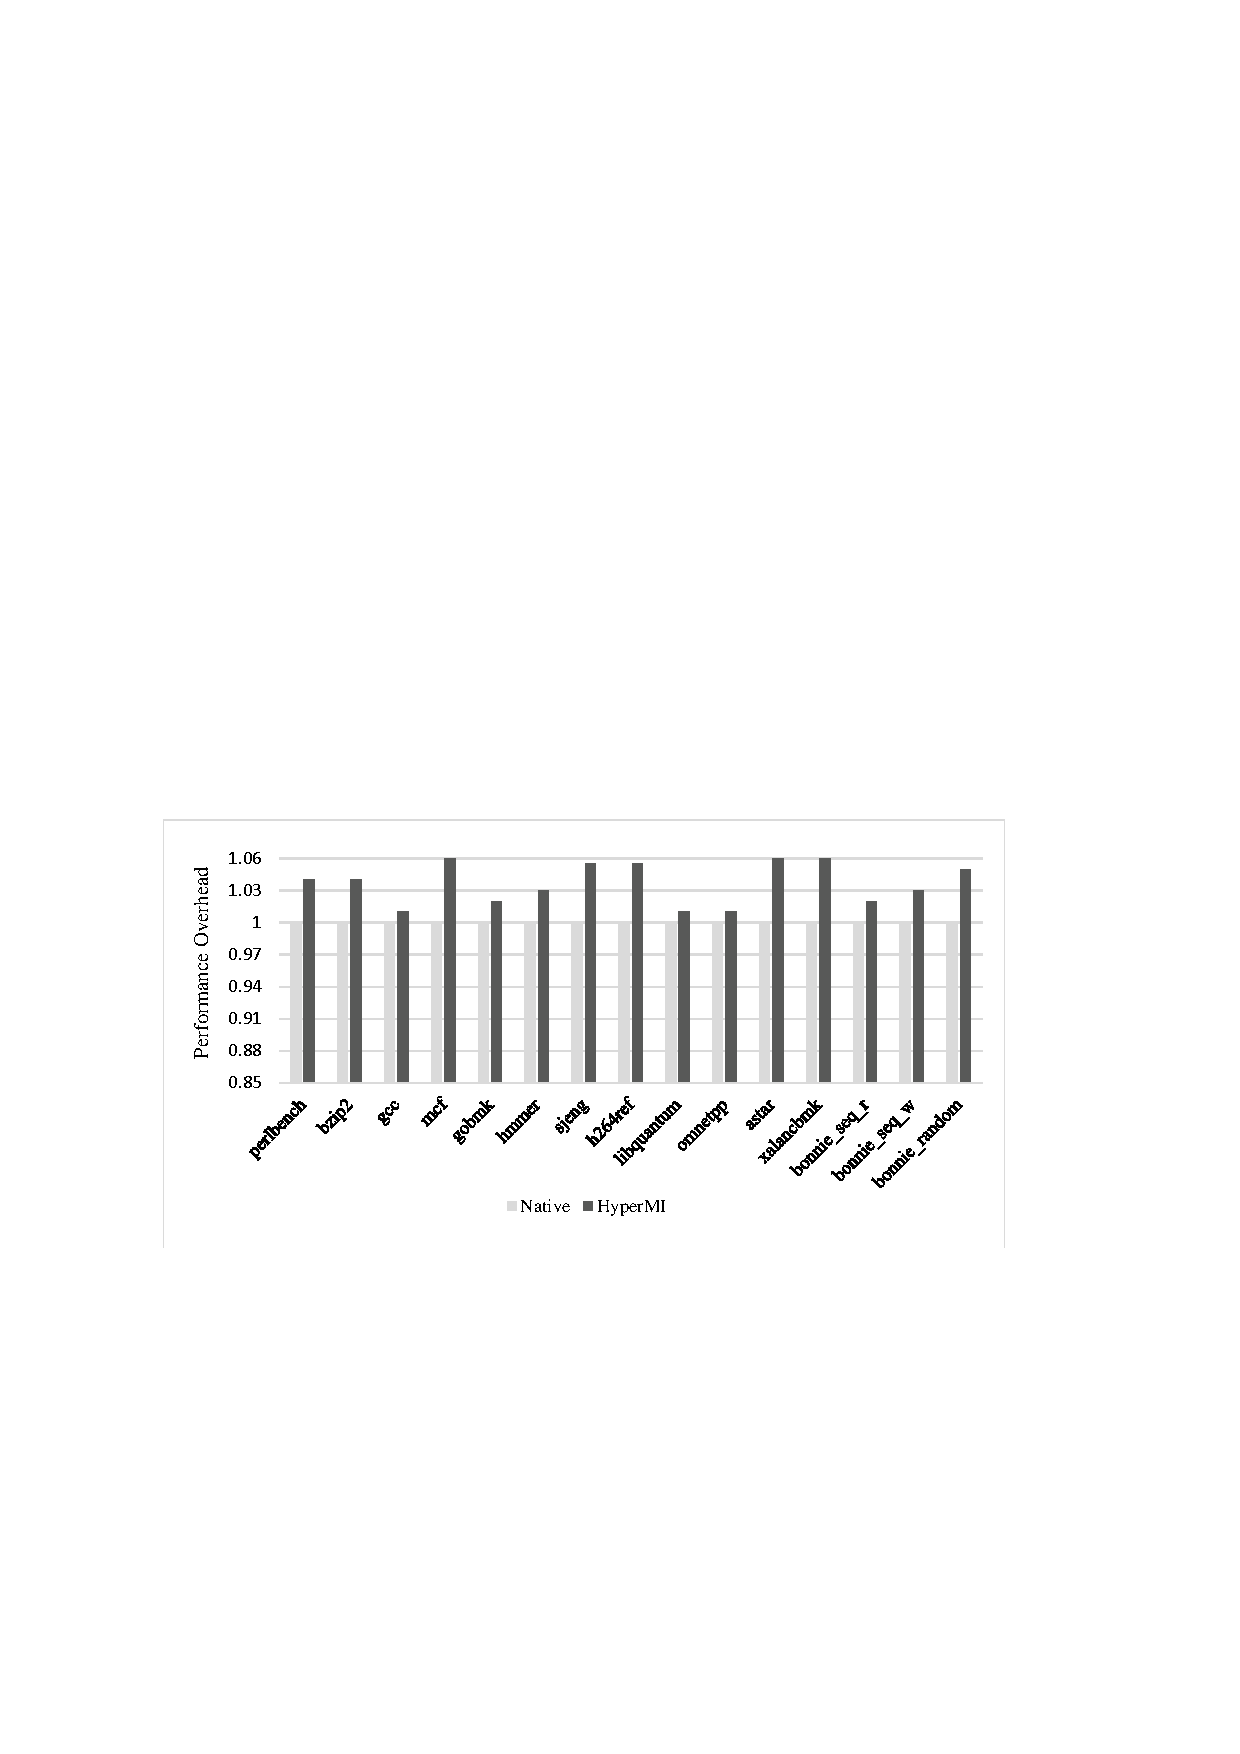
\includegraphics[width=0.8\linewidth]{IMG/performance.pdf}
    \caption{Performance Overhead}%
    \label{fig5}
\end{figure}
%FIXME 修改图为HyperPS

\subsection{Performance Evaluation}
In this section, we evaluate the performance of our HyperPS prototype. all the experiments were conducted on a physical server with a 2.0 GHz 64 core Intel processor and 32 GB memory. The Host system runs Ubuntu 16.04 LTS with kernel version of 4.4.1. We created more than five virtual machines. The guest is configured with 1GB of memory and runs Ubuntu 16.04 LTS Service with a kernel version of 4.4.1. 

%All experiments are done on a server with 64 cores and 32 GB memory, running at 2.0 GHz and 5 VMs. 

In our prototype, the HostOS kernel is modified so that HyperPS Space is initialized during the boot up sequence. This includes creating a new memory page table for HyperPS, allocating memory pages, as well as creating Page-Mark table and VM-Mark table. This process introduces security verification for pages according to Page-Mark Table, and security accessing to VMCS in HyperPS Space during VM Exit/Entry sequence.
The kernel is modified to place hooks upon some functions.
%control registers, accessing VMCS operations, and accessing EPT operations。
% in order to achieve HyperPS Space, VM Monitoring and VM Isolation.
% The contorl flow jumps to HyperPS Space through the switch gate. 
% introducing worlds switching overhead using switch gate.

%We do not directly compare HyperPS with previous software approaches, as they cannot support all functions simultaneously. 
To evaluate the performance of HyperPS, we experimented with SPECCPU 2006, Bonnie++ and HyperBench. The SPECCPU 2006 measure HyperPS's impact to compute-intensive workloads, such as gcc; The Bonnie++ quantifies the performance overhead introduced by HyperPS for file systems; and the HyperBench measure the overall cloud performance under HyperPS, especially impact to the KVM Hypervisor.
All the experiments were repeated fifty times in the cloud environment with HyperPS and in the original cloud environment (the baseline).
In these fifty experiments, we set up different workloads (different numbers of guest VMs with different memory size) to simulate different environments in the real cloud environment. 
Besides, we also measured the VM load time to evaluate the impact to VM initialization.
The average reuslts of all the experiments are reported. 


% All the experiments were repeated ten times and the average results are reported.

% In order to assess the effectiveness of all aspects of HyperPS, we conduct a set of experiments to evaluate the performance impact imposed by HyperPS against an original KVM system (the baseline). We run two groups of experiments, compare the performance overhead including benchmarks performance overhead , cloud performance overhead and VM load time.
% For simplicity, we only present the performance evaluation on a server with 64 cores and 32 GB memory, running at 2.0 GHz and guest VM with 2 virtual cores. The version of the hypervisor and guest VM is 3.10.1.
% Different experiments are based on different numbers of guest VMs with different memory size. Both the original hypervisor and HyperPS systems have the same configuration except the protection supported by HyperPS. The deviation of these experiments is insignificant. All the experiments are replicated fifty times and the average results are reported here.



\textbf{Benchmarks Performance}
%All experiments are done on a server with 64 cores and 32 GB memory, running at 2.0 GHz and 5 VMs. 
% In order to obtain the impact of HyperPS on the whole system, we measure HyperPS with microbenchmarks and application benchmarks.
% We use one guest VM with 1 GB memory size.
%All experiments are done 50 times and results are from the average.
We firstly expermiment with SPECCPU 2006 to measure the performance overhead introduced by HyperPS.
SPECCPU 2006 consists of several compute-intensive benchmarks, strssing the system's processor and memory subsystems. 
% for compute-intensive applications.
The experiment results are list in Figure \ref{fig5}. As shown in this figure, for the majority of these applications, such as perlbench, bzip2, gcc, gobmk, libquantum and ometpp, 
HyperPS introduced at most 3\% performance overhead. 
However, there are still several benchmarks, such as mcf, astar and xalancbmk whose results are higher than everage, 
They caused a performance loss of 6\%. 
Most of these workloads have large and fluctuating memory footprints. 
It's not surprising as the HyperPS takes over physical memory management. Frequent memory request incurs HyperPS involvement to index the Page-Mark Table and verify the legality of EPT paging-structure updates.
% handles Page-Mark structure and verifies the legality of page mapping when EPT updates.
We can conclude that, for most compute-intensive application without large memory footprints, HyperPS has the similar performance as the baseline cloud environment. 
For applications with large memory footprints, 
We believe that these performance impact is completely acceptable to trade this performance loss for higher security.
% These performance impact is still acceptable. Besides, we also achieve

% The high overhead related to memory allocation
% We believe that it is completely acceptable to trade this performance loss for higher security.
% These performance impact is still acceptable
% but they are acceptable

% We can conclude that, for most compute-intensive application without large memory footprints,
% This result
% HyperPS has the similar performance as the baseline cloud environment.
% HyperPS introduced at most 3\% performance overhead.
% most of the SPECCPU 2006 workloads

% To better understand the factor causing the performance overhead, we experiment with compute-bound benchmark (SPEC CPU2006 suite) and one I/O-bound benchmark (Bonnie++) running upon original KVM and HyperPS in a Linux VM. The experiment result described in Figure \ref{fig5}(the last three groups) shows a relatively low cost. Most of the SPEC CPU2006 benchmarks (the first twelve groups) show less than 6\% performance overhead. It's not surprising as there are few OS interactions and these tests are compute-bound. Mcf, astar, and xalancbmk with the highest performance loss allocate lots of memory. HyperPS handles Page-Mark structure and verifies the legality of page mapping when EPT updates. This can incur worlds switching which involves controlling register access and incur VM exit which involves EPT updating.
% and fewer TLB flushes with PCID technique because the two worlds are at the same privileged layer.

We then experiment with Bonnie++ to measure the performance overhead introduced by HyperPS to file systems. 
Bonnie++ sequentially reads/writes data from/to a particular file in different ways. The read/write granularity varies from a character to a block. Furthermore, we also test the time cost of the random access. 
% In our experiments, we specified the file size
% Bonnie++ performed a series of test operations on a file with a known file size.
In our experiments, the target file which Bonnie++ performs a series of test operations on is 1000MB size. 
% We used Bonnie++ to perform sequential read, write and random access to the file.
Figure \ref{fig5} shows the Bonnie++ measurement results which show the performance overhead on the file system is acceptable too. 
The performance loss of sequential read, write and random access is 2\%, 3\% and 5\%, 
Actually, HyperPS does not interpose much on memory operations for I/O data. 

\iffalse
% The performance loss of
The result
used Bonnie++ 
% We created a file which as 1000MB as the
For Bonnie++, we choose a 1000 MB file to perform the sequential read, write and random access. The performance loss of sequential read, write and random access is 2\%, 3\% and 5\%, 
These performance loss it not high.
the main reason is that HyperPS has no extra memory operations for I/O data. The performance result shows that HyperPS introduces trivial switch overhead of two worlds and trivial overhead of memory isolation of VMs.
\fi

%{\bfseries\textbf\centering{Page-Mark Table}}
\begin{table}
\centering
\caption{execution time of vm operation(s).}\label{tabvm}
%\begin{tabular}{|c{1cm}|c|c|}
\begin{tabular}{p{2cm}|p{1.8cm}|p{2cm}}
\hline
{\itshape\bfseries  Test Case} & {\itshape\bfseries VM Create} & {\itshape\bfseries VM Destroy} \\
\hline
No\_HyperPS & 11.79 s &  1.75 s\\
\hline
With\_HyperPS & 12.97 s & 1.89 s\\ 
\hline
Efficiency & 1.1 & 1.08 \\
\hline
\end{tabular}
\end{table}


HyperBench is a benchmark suit that focuses on measuring cloud performance, especially on measuring on HostOS/Hypervisor's capabilities. 
The HyperBench designs 15 hypervisor benchmarks covering CPU, memory, and I/O. The operation in each benchmark triggers hypervisor-level events, which examines the platform's ability in the target area. We used HyperBench to evaluate the performance loss introduced by HyperPS to the HostOS/Hypervisor.
The results are shown in Figure \ref{}. For half of the test cases, HyperPS does not introduce performance overhead or little performance loss which is less than 1 percent. 
Inter-Processor Interrupt (IPI) is a special type of interrupt by which one processor may interrupt another in a multiprocessor system. 
HyperPS introduces 4\% performance overhead in this test suit. 
The virtual IPI delivery requires two VM exits and need to write to VMCS. Because the VMCS has been removed in the Normal Space, access to VMCS requires the involvement of HyperPS.  
HyperPS also poses a higher impact on the cold-access test suit (about 5 percent). 
As mentioned above, the KVM constructs EPT with page faults. Data accessed in the cold-access benchmark is not loaded into physical memory in advance, thus, the EPT does not maps these data before. In our prototype, HyperPS interposes EPT paging-structure initialization and EPT Page Fault handle procedure. 
All EPT Updates are completed in the HyperPS Space. This is the reason why HyperPS introduced performance loss in this test suit. 
As shown the Figure \ref{}, compared with the cold-access benchmark, the performance overhead introduced by HyperPS in the hot-access benchmark is obviously smaller. 
set-pt is another benchmark that operates on EPT. HyperPS introduced about 4 percent performance overhead than the baseline because all EPT operations are hooked into the HyperPS Space. 
    



\textbf {VM Load Time}
% and World Switch Overhead}
The load time of a VM is a critical aspect of performance to be considered because it influences user experience. We design experiments to evaluate the performance impact of HyperPS for VM loading.
% Experiments are done with 4 VMs, each guest VM is with different memory sizes from 512MB to 4GB.
 %As expected, the VM booting time in HyperPS increases as the memory sizes increase, and the growth amplitude are more and much larger due to the world switch and page tracking caused by frequent memory allocation.
 We measure the impact of completely booting and shutdowning a VM (configured with 2 VCPU and 512MB memory). As Table \ref{tabvm} shown, the booting time is suffered a 1.1 times slowdown under HyperPS, shutdown time is suffered a 1.08 times slowdown, due to the extra overhead of worlds switching and Page-Mark table accessing in HyperPS Space. Such overhead is worth for HyperPS.
